\setchapterpreamble[u]{\margintoc}
\chapter{Proof-by-Action in Practice}
\labch{advanced}

The chapter is organized as follows: \refsec{edukera} studies a proof of a small
logical riddle in Actema, highlighting some benefits of our approach compared to
textual systems.

\section{A More Advanced Example}\labsec{edukera}

It is too early to perform a detailed case study comparing our approach
to interactive theorem proving with others --- tactic-based,
declarative, {\em etc}\dots~This is due primarily to the fact that
our prototype is not mature enough; it cannot handle lemmas and
implements a limited formalism. However some examples allow to get a
glimpse of specificities and possible advantages of proofs by actions.

One such example is a small logical riddle, which we borrow from a
textual educational system, Edukera~\sidecite{edukera}. One considers a
population of people, with at least one individual $h$, together with a
single function $\mother$ and one predicate $\rich$. The aim is to
show that the two following assumptions are incompatible:
\begin{itemize}
\item[(1)] $\forall x. \neg\rich(x)\lor \neg\rich(\mother(\mother(x)))$,
\item[(2)] $\forall x. \neg\rich(x) \limp \rich(\mother(x)).$
\end{itemize}
The original goal thus corresponds to the illustration of \reffig{edukera}.

\begin{figure*}
  \fbox{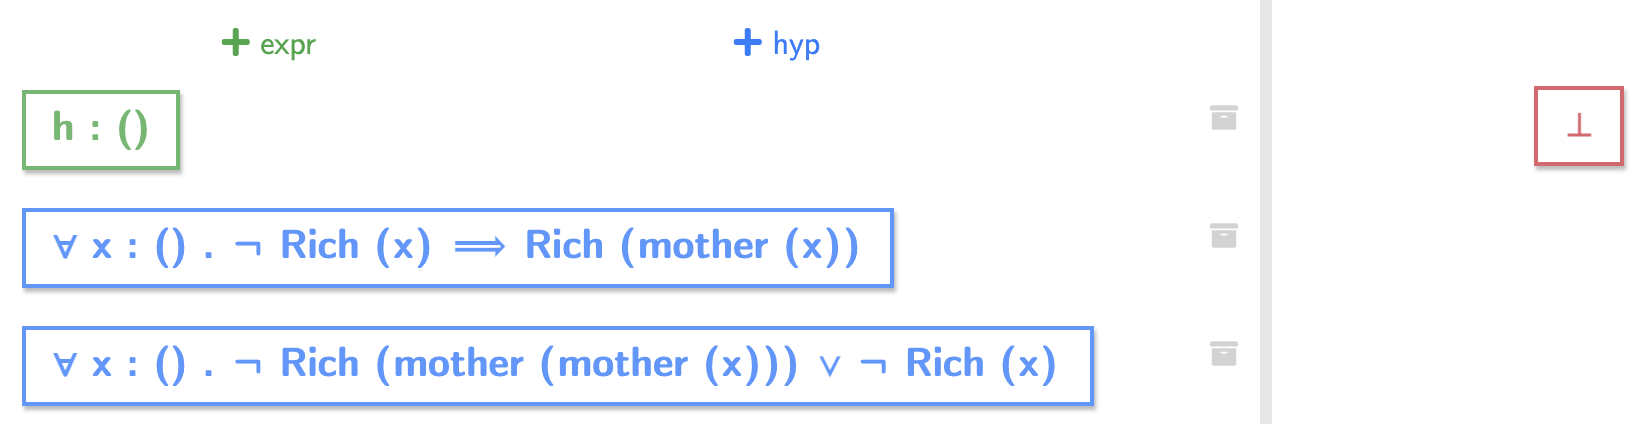
\includegraphics[width=1.3\textwidth]{edukera.png}}
  \caption{The beginning of an example due to Edukera}
  \labfig{edukera}
\end{figure*}

It is quite natural to approach this problem in a forward manner, by starting
from the hypotheses to establish new facts. And a first point illustrated by
this example is that DnD actions allow to do this in a smooth and precise
manner. A possible first step is to bring $h$ to the first hypothesis, to obtain
a new fact:

\medskip
$(3) ~\neg\rich(h)\lor \neg\rich(\mother(\mother(h))).$
\medskip

\noindent Double clicking on this new fact yields two cases:
\begin{itemize}
 \item[(4)~] $ \neg\rich(h)$,
 \item[(4')] $ \neg\rich(\mother(\mother(h)))$.
 \end{itemize}
Let us detail how one solves the
second one.

By bringing 
$\neg\rich(\mother(\mother(h)))$ on the premise of $\forall
x. \select{\neg\rich(x)} \limp \rich(\mother(x))$
one obtains

\medskip
$(6) ~\rich(\mother(\mother(\mother(h)))).$
\medskip

The next step is a good example where the DnD is useful. By bringing
this new fact to the right-hand part of

\medskip
$(1)~\forall x. \neg\rich(x)\lor \neg\select{\rich(\mother(\mother(x)))}$
\medskip

\noindent
one immediately obtains a new fact

\medskip
$(7) ~\neg{\rich(\mother(h))}$.
\medskip

\noindent In other proof systems, this last step requires a somewhat intricate
tactic line and/or writing down at least the statement of the new fact.

One can then finish the case by combining $(7)$ and $(2)$ which yields
$$\rich(\mother(\mother(h)))$$ contradicting $(4')$. These two last steps each
correspond to a simple DnD. The other case, $\neg\rich(h)$, is quite similar.

Such a simple example is not sufficient to provide significant
metrics. Note however that once a user has understood the proof, the
riddle is routinely solved in less than a minute in Actema, which
seems out of reach for about any user in a tactic based prover. At
least as important is the fact that the proof can be performed without
typing any text, especially no intermediate statement. 
